%! TEX root = ../main.tex
\documentclass[../main.tex]{subfiles}

\begin{document}

\subsection{Fenditura $a = \qty{0.04}{\milli\metre}$}

\begin{figure}[ht!]
    \centering
    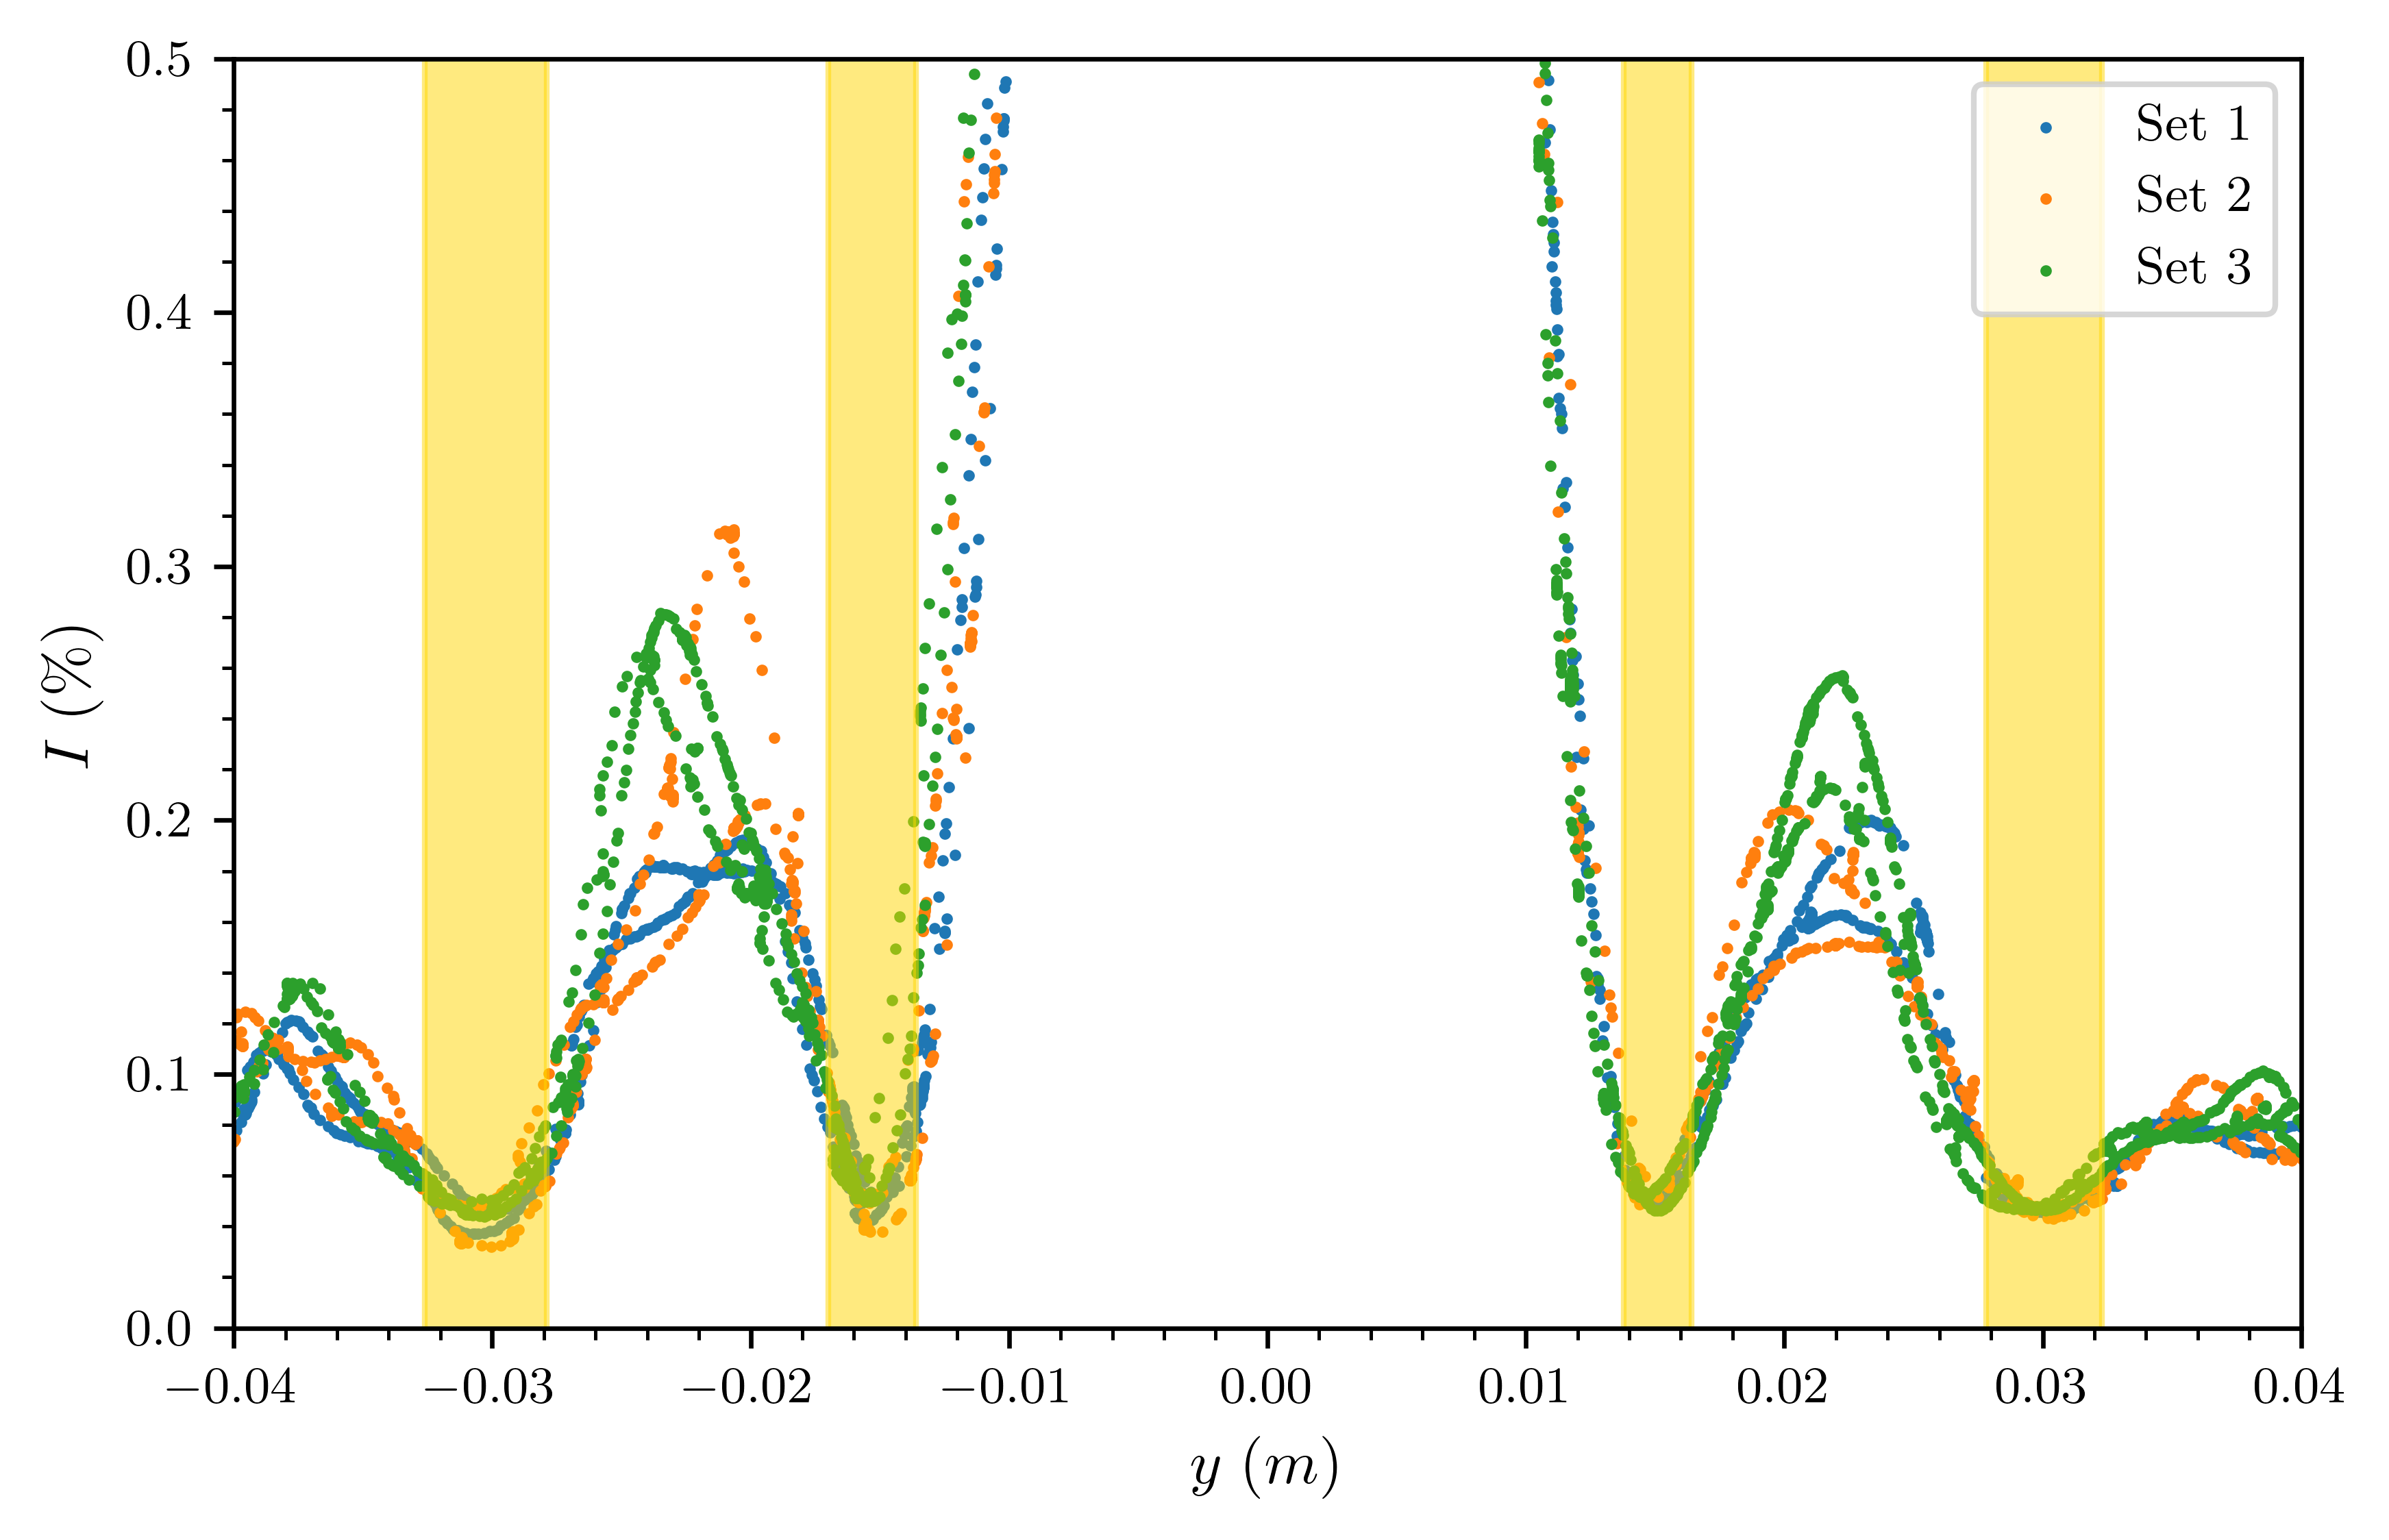
\includegraphics{min_0.04.png}
    \caption{Intensità luminosa $I$ in funzione della posizione $y$ del sensore (in metri) per la fenditura a $\qty{0.04}{\mm}$. I dati dei set 1 e 3 risultano quasi simmetrici, mentre il set 2 è visibilmente asimmetrico. In figura sono segnati i minimi ricavati graficamente con i relativi errori. Qui si considera un errore di posizione di $\qty{0.5}{\mm}$.} % todo: aggiungere qualcosa in più alla descrizione, trovare forse un motivo migliore per l'errore di 1mm
    \label{fig:minimi 0.04}
\end{figure}

Le posizioni dei minimi ottenute sono le seguenti:

\begin{table}[ht!]
    \centering
    \caption{}
    \import{../tables/}{mins_0.04.tex}
    \label{tab:minimi 0.04}
\end{table}

Intersecando le barre d'errore dei valori ottenuti si ha $a = \qty{0.043+-0.003}{\mm}$.

% Prendendo in considerazione la somma delle barre d'errore dei valori ottenuti $a = \qty{0.043+-0.004}{\mm}$.

% Facendo una media pesata dei valori ottenuti si ha $a = \qty{0.0424+-0.0012}{\mm}$. %? media o intersezione

\begin{figure}[ht!]
    \centering
    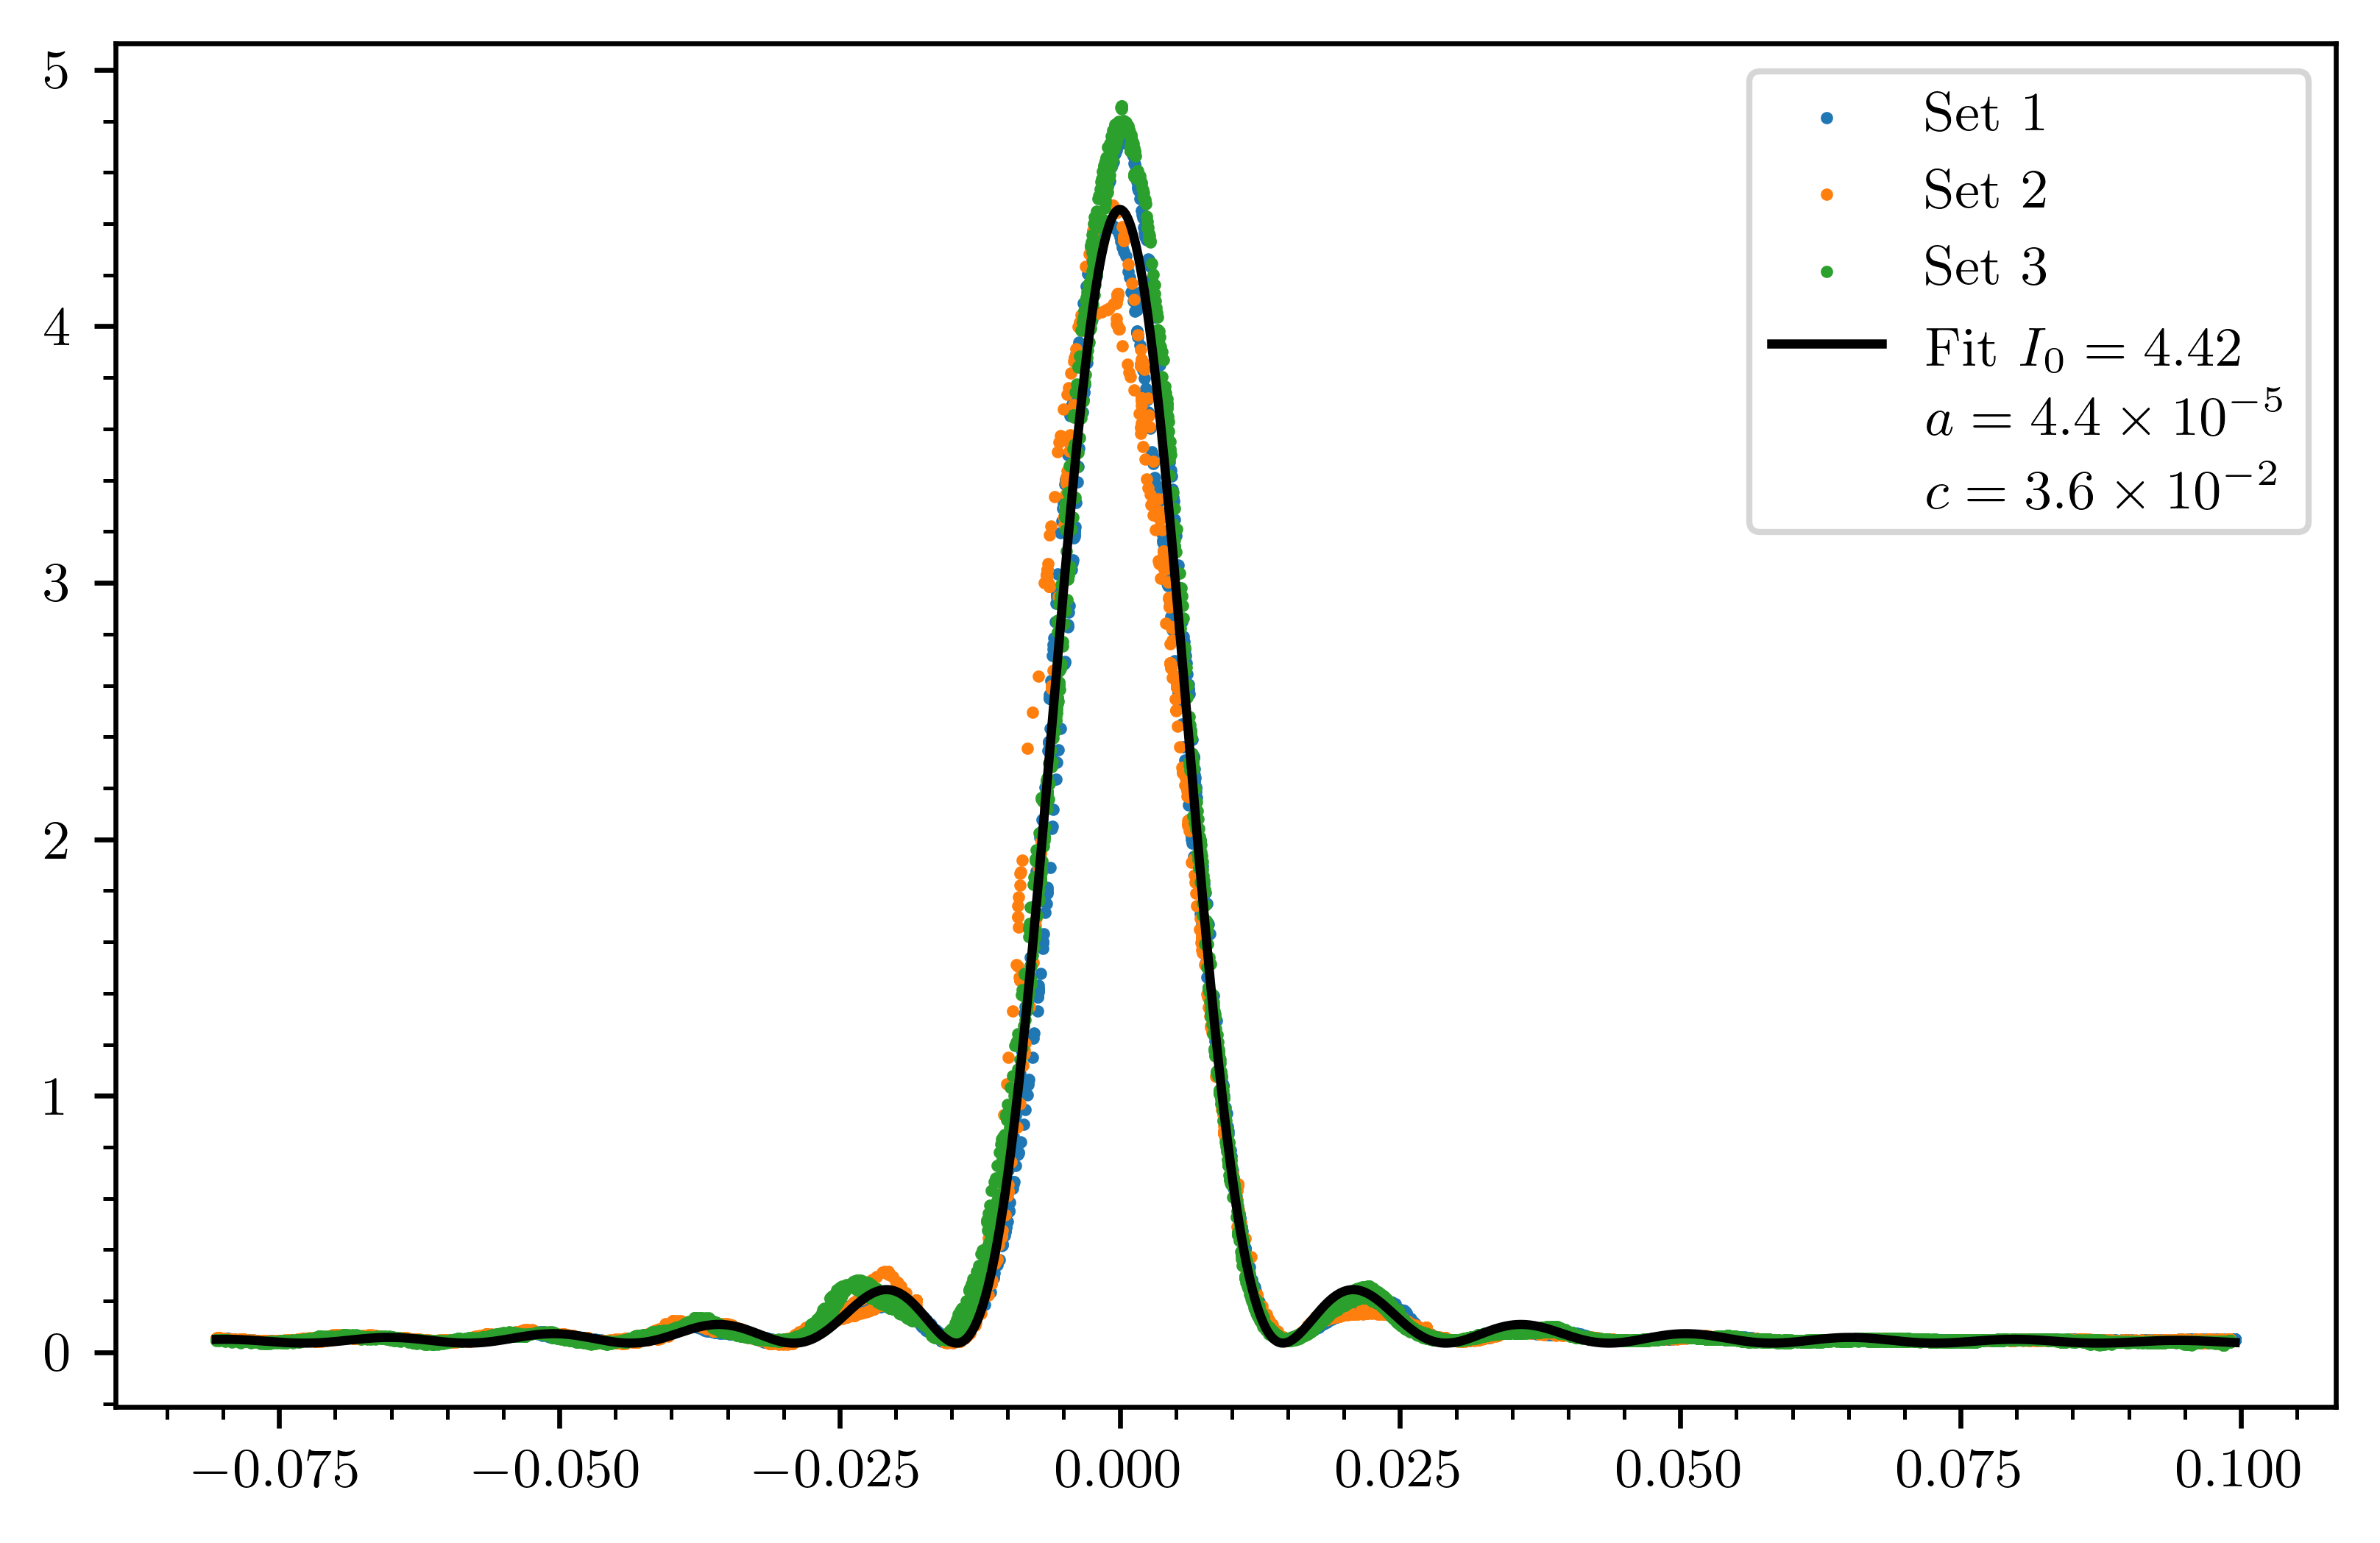
\includegraphics{fit_0.04.png}
    \caption{Intensità luminosa $I_{0}$ in funzione della posizione $y$ del sensore (in metri) per la fenditura a $\qty{0.04}{\mm}$. In figura è riportato il fit fatto utilizzando l'\autoref{eq:fit}. I valori dei parametri ottenuti sono $I_{0} = \num{4.42+-0.4}$, $a = \qty{4.4+-0.5e-5}{\mm}$ e $c = \num{3.60+-0.01}$. }
    \label{fig:fit 0.04}
\end{figure}

I valori di $a$ ottenuti dal grafico e dal fit risultano compatibili con il valore teorico.

Nel grafico seguente si confrontano i set ottenuti con le diverse aperture del sensore:

\begin{figure}[ht!]
    \centering
    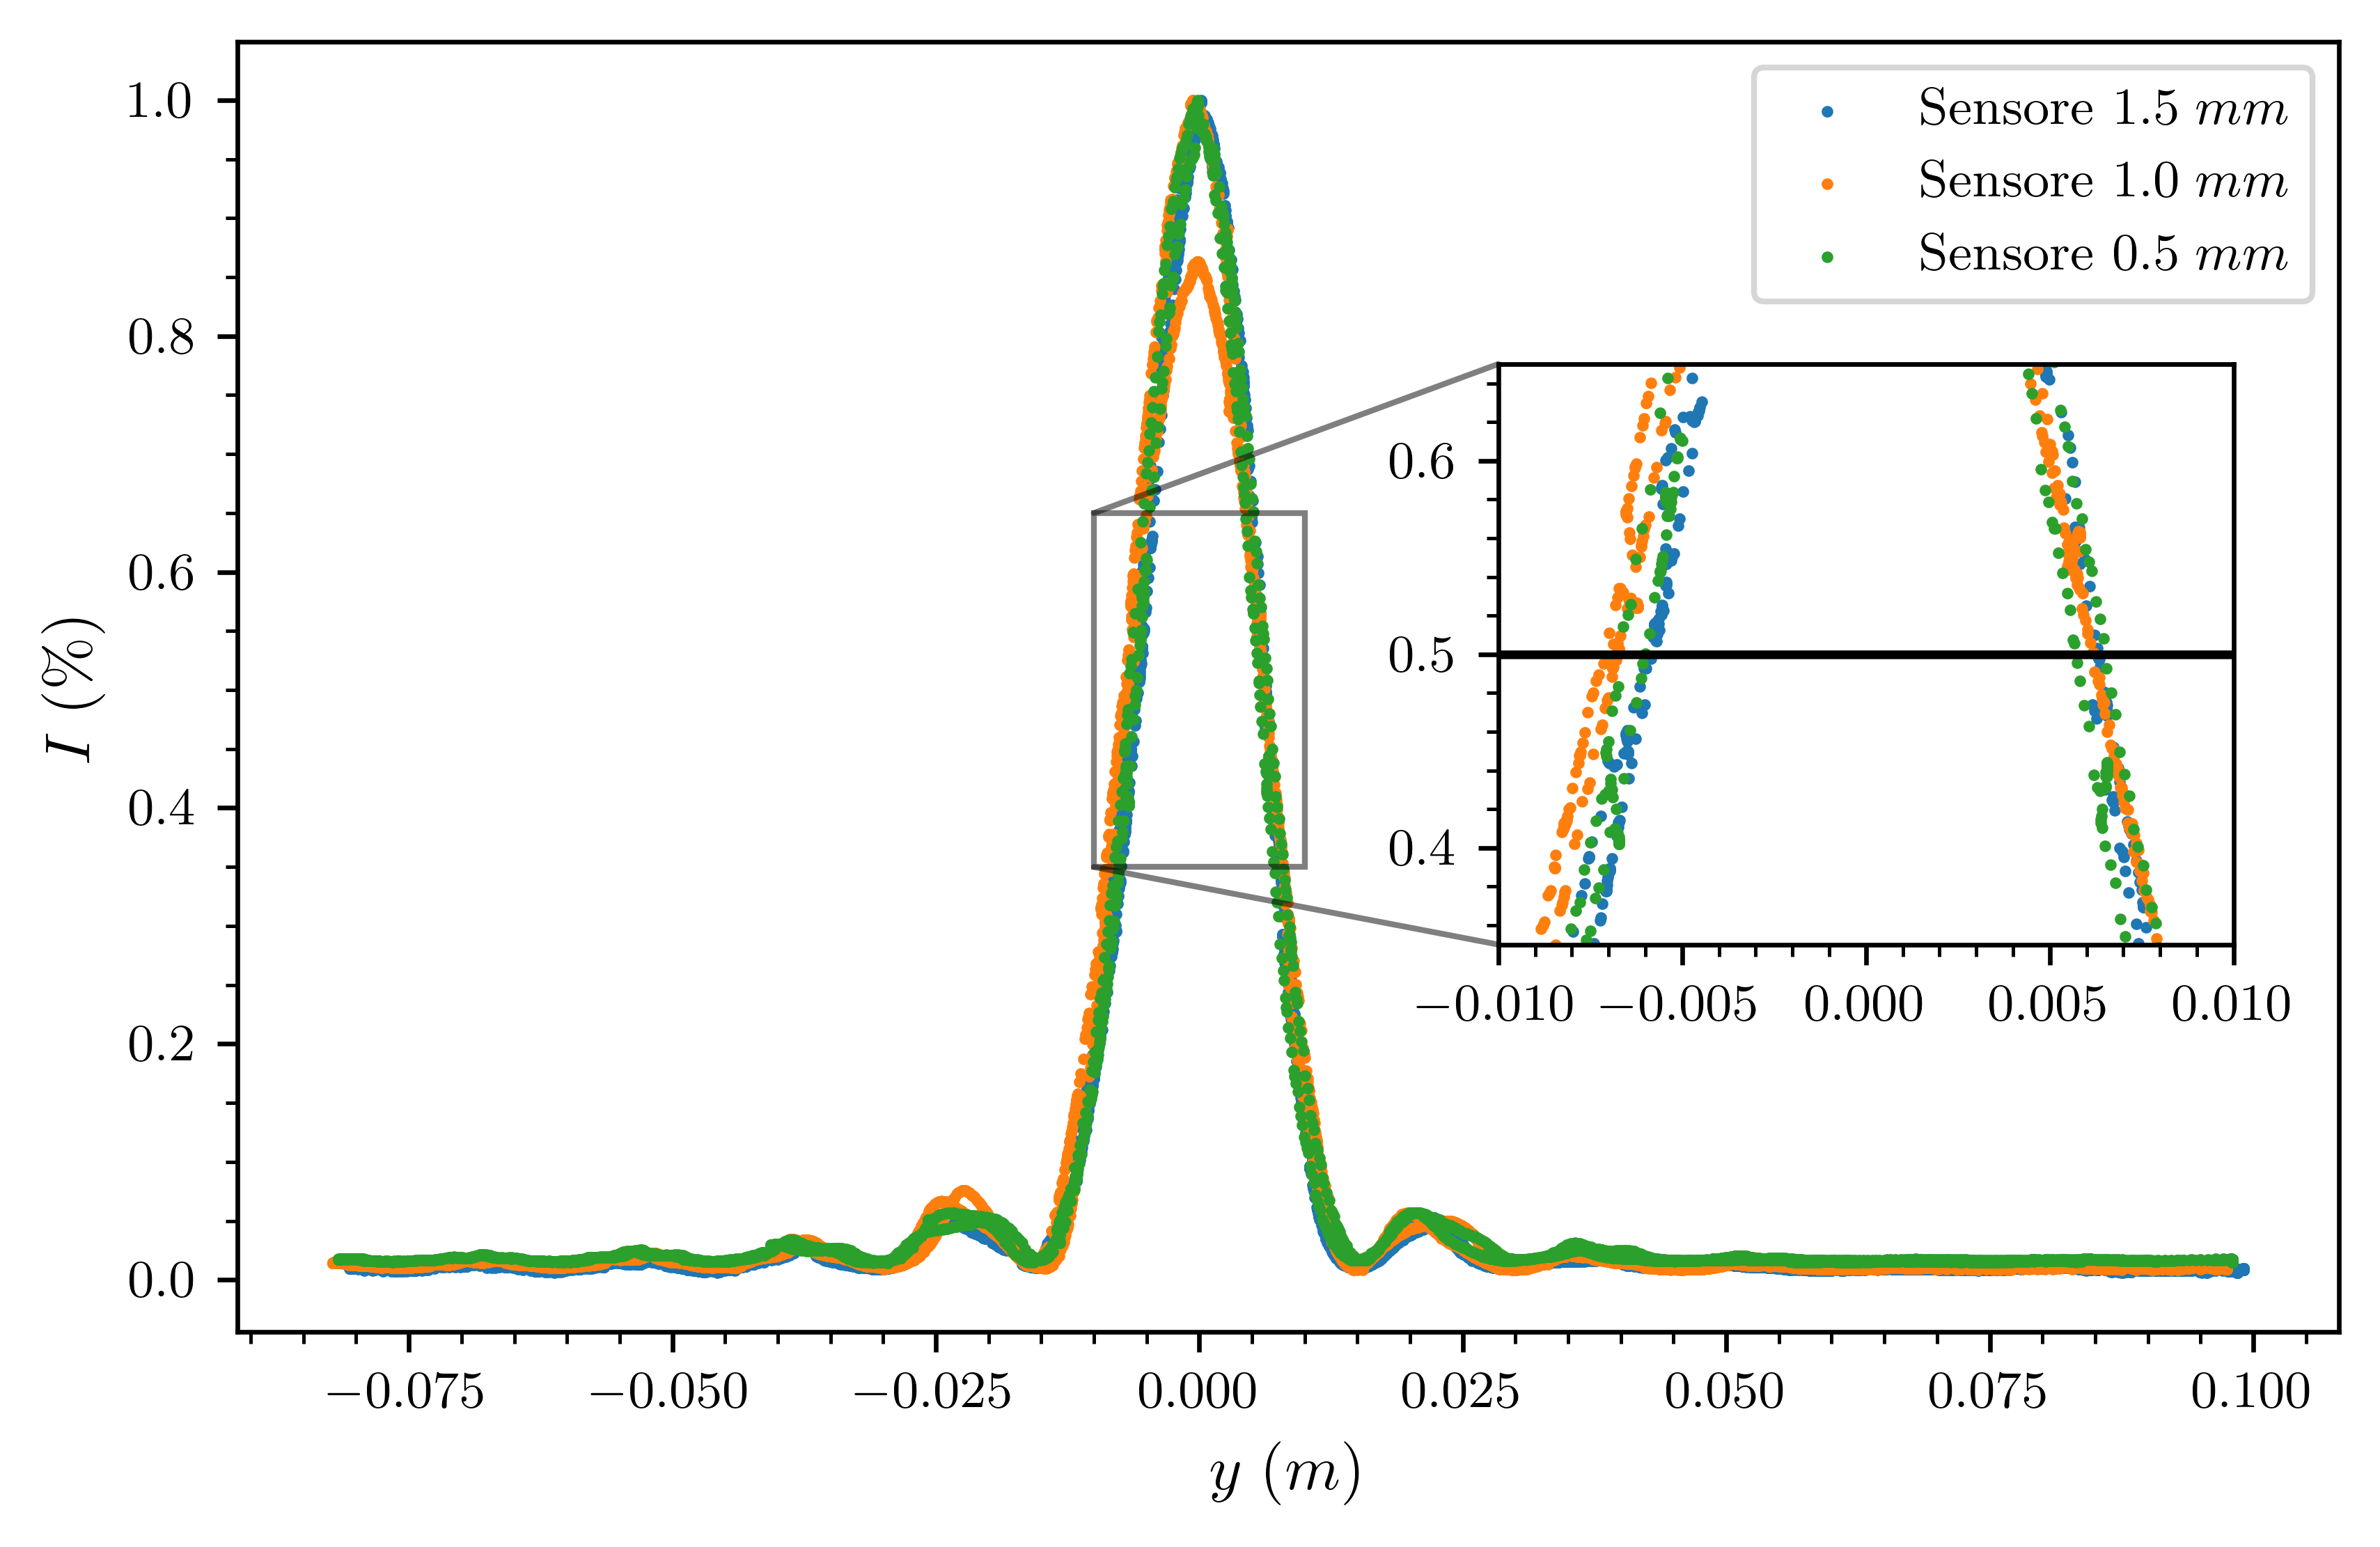
\includegraphics{sensor_0.04.png}
    \caption{}
    \label{fig:sensore 0.04}
\end{figure}

\begin{figure}[ht!]
    \centering
    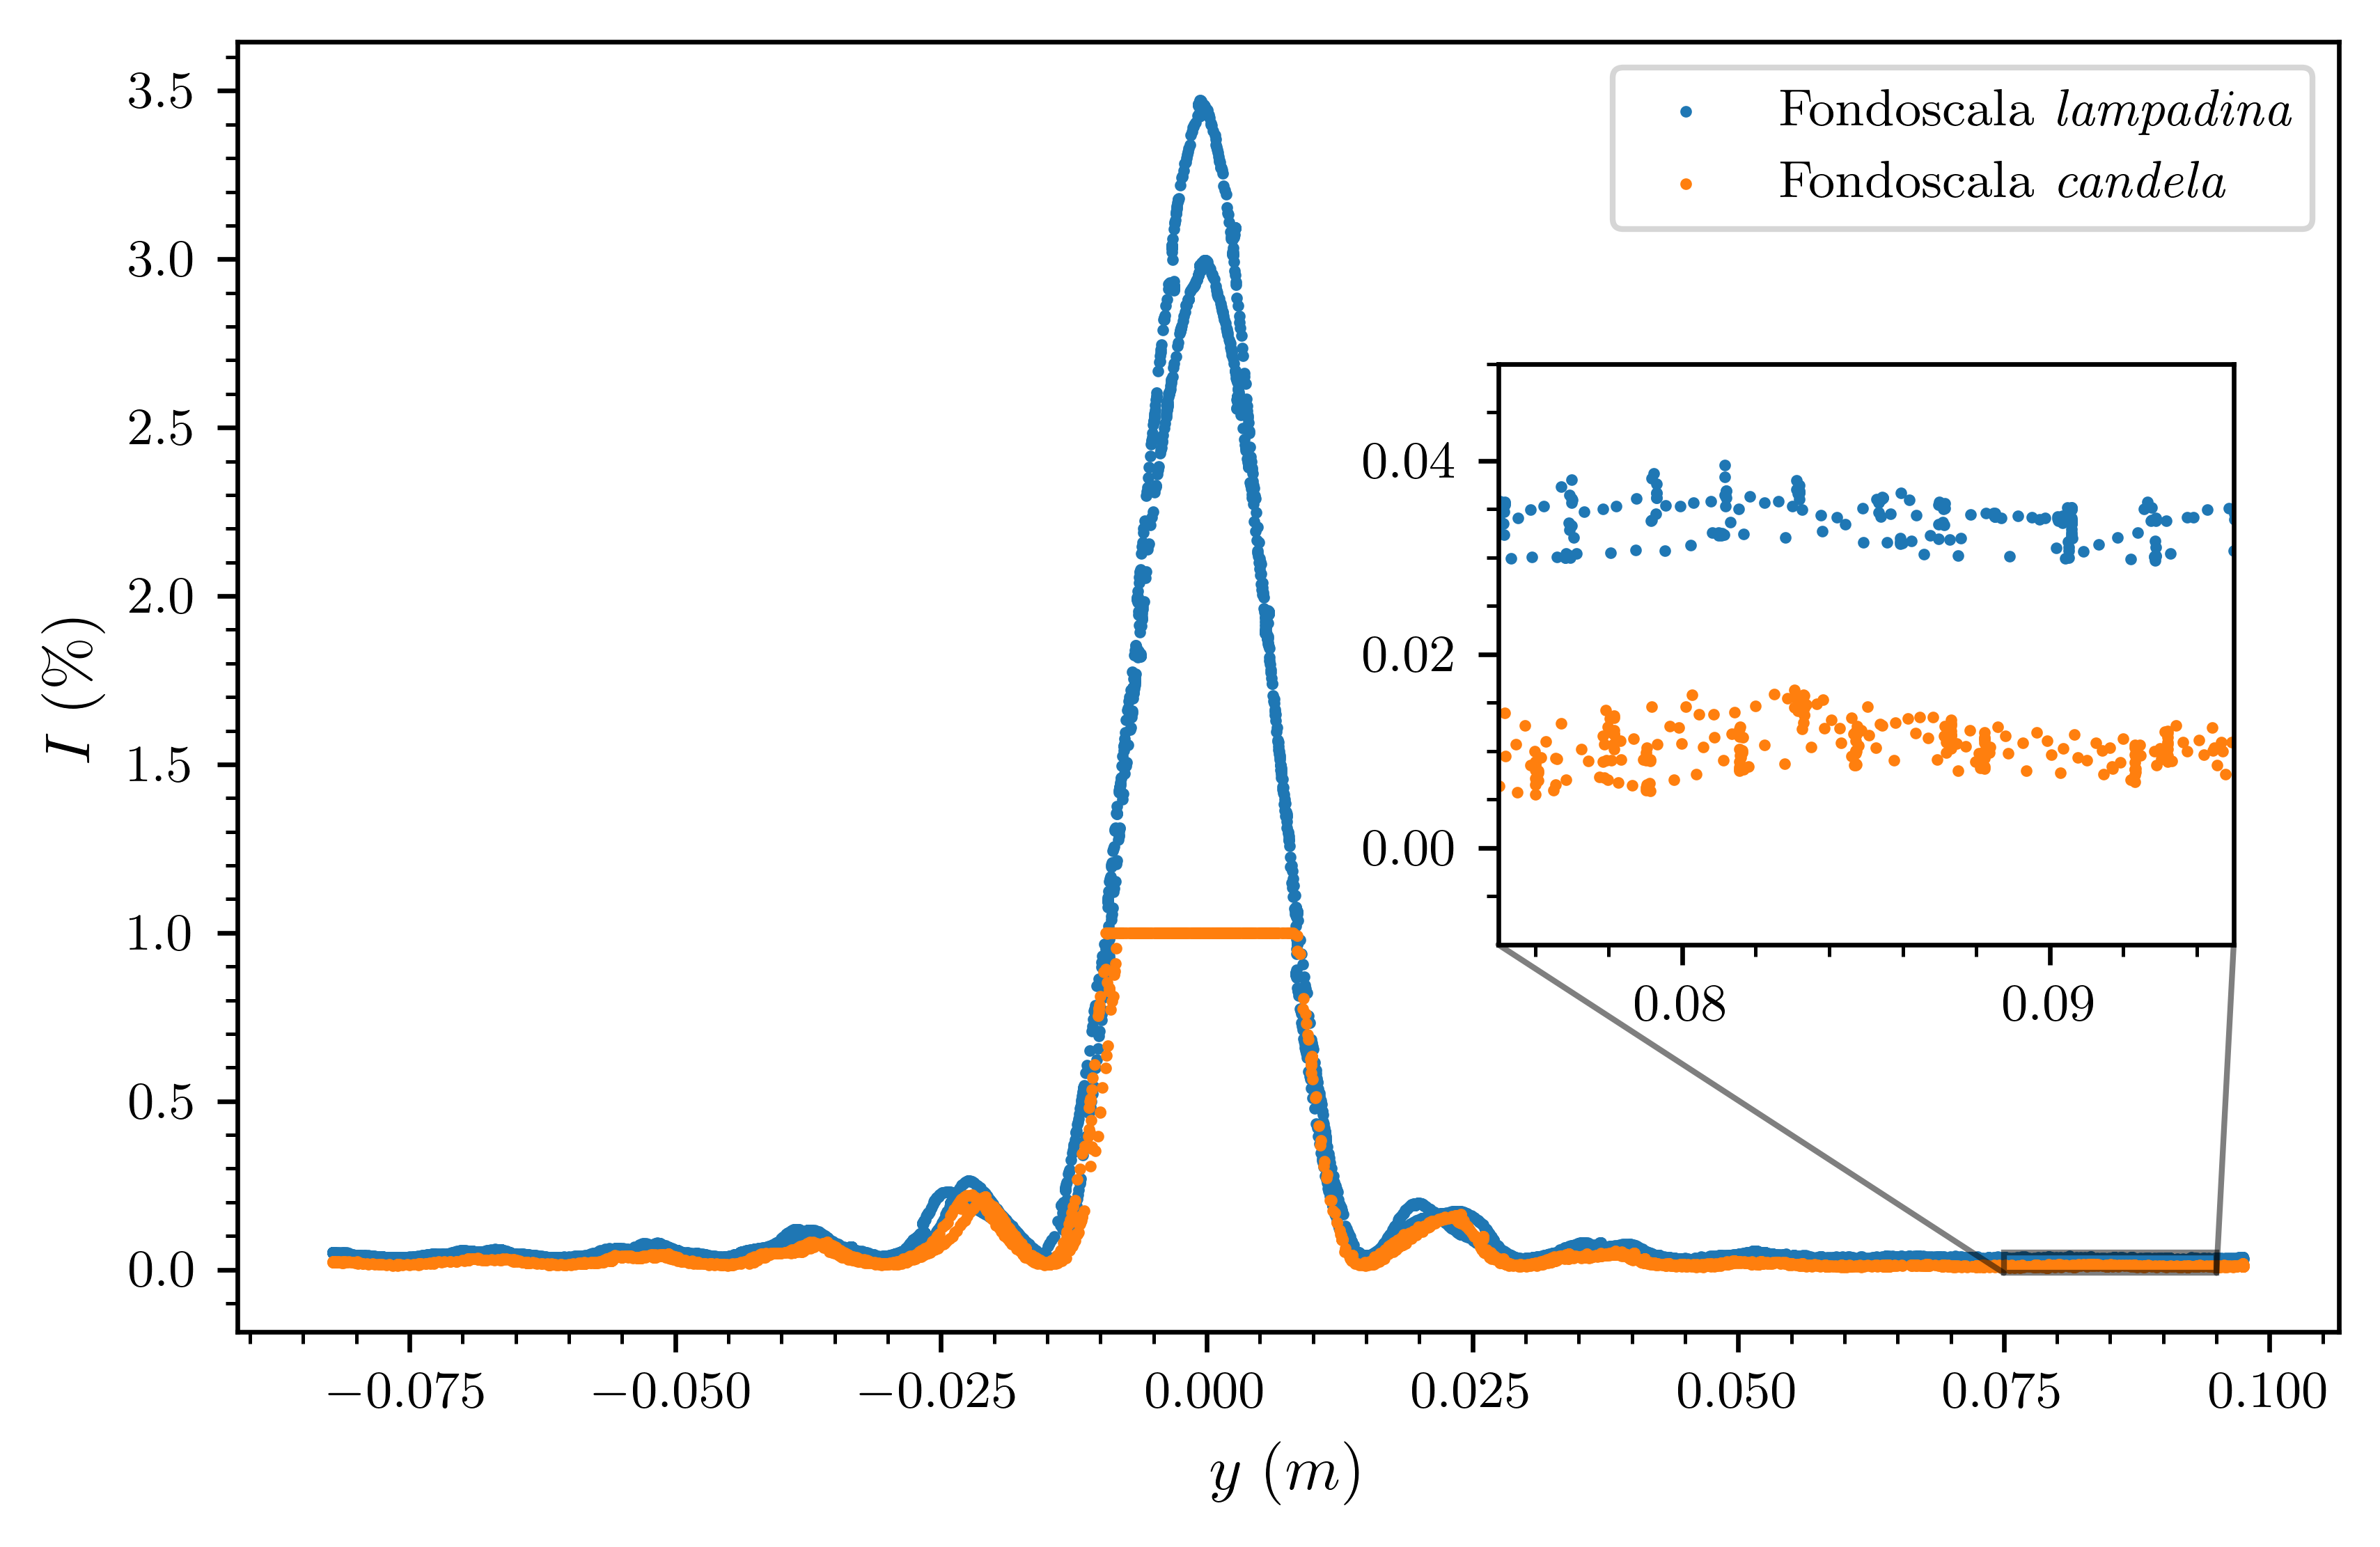
\includegraphics{scale_0.04.png}
    \caption{Grafico dell'intensità in funzione della posizione dove si confrontano i due fondoscala, con uno zoom sulla coda del grafico per evidenziare la diminuzione di rumore data dal fondoscala più piccolo.}
\end{figure}

\end{document}